\documentclass[aspectratio=169]{beamer}
\usepackage{hyperref}
\usepackage[T1]{fontenc}
\usepackage[spanish]{babel}
\usepackage{csquotes}
\usepackage{tribhuvan}

\usepackage{latexsym,amsmath,xcolor,multicol,booktabs,calligra}
\usepackage{graphicx,pstricks,listings,stackengine}

\author{Rodrigo Pérez Rodríguez}
\title{Tecnologías Robóticas para la Discapacidad Intelectual}
\subtitle{Control de comportamientos y máquinas de estados finitos}
\date{}
\setbeamertemplate{date}{}

\AtBeginSection[]{
  \begin{frame}[plain]
    \vfill
    \begin{center}
      {\LARGE\bfseries \insertsectionhead}
    \end{center}
    \vfill
  \end{frame}
}
\AtBeginSubsection[]{}

\def\cmd#1{\texttt{\color{red}\footnotesize $\backslash$#1}}
\def\env#1{\texttt{\color{blue}\footnotesize #1}}
\definecolor{deepblue}{rgb}{0,0,0.5}
\definecolor{deepred}{rgb}{0.6,0,0}
\definecolor{deepgreen}{rgb}{0,0.5,0}
\definecolor{halfgray}{gray}{0.55}

\lstset{
    basicstyle=\ttfamily\small,
    keywordstyle=\bfseries\color{deepblue},
    emphstyle=\ttfamily\color{deepred},
    stringstyle=\color{deepgreen},
    numbers=left,
    numberstyle=\small\color{halfgray},
    rulesepcolor=\color{red!20!green!20!blue!20},
    frame=shadowbox,
}

\begin{document}

\begin{frame}
    \titlepage
\end{frame}

\begin{frame}
    \tableofcontents[sectionstyle=show,subsectionstyle=show/shaded/hide,subsubsectionstyle=show/shaded/hide]
\end{frame}

%=================================================
\section{Control de comportamientos}
%=================================================

\begin{frame}{Control de comportamientos en robots}
\small
\begin{itemize}
  \item Objetivo: conseguir respuestas robustas, seguras y repetibles en situaciones reales.
  \item Un robot autónomo necesita:
  \begin{itemize}
    \item percibir el estado del entorno,
    \item decidir que hacer,
    \item ejecutar acciones y corregir errores.
  \end{itemize}
  \item En cursos introductorios suele aparecer primero control reactivo y control clásico.
  \item En este tema introducimos \textbf{máquinas de estados finitos (FSM)} como alternativa para estructurar comportamiento.
\end{itemize}
\end{frame}

\begin{frame}{Sistemas reactivos: fortaleza y límite}
\small
\begin{itemize}
  \item Regla básica: \textit{si pasa X, hago Y}.
  \item Ventajas:
  \begin{itemize}
    \item simples de implementar,
    \item respuesta rápida,
    \item bajo coste computacional.
  \end{itemize}
  \item Limitaciones:
  \begin{itemize}
    \item escalan mal al crecer escenarios,
    \item aparecen vacíos y solapes de control,
    \item cuesta explicar y mantener la lógica global.
  \end{itemize}
\end{itemize}
\end{frame}

%=================================================
\section{Máquinas de estados finitos}
%=================================================

\begin{frame}{FSM como arquitectura de decisión}
\small
\begin{columns}[T,onlytextwidth]
  \begin{column}{0.58\textwidth}
    \begin{itemize}
      \item Una FSM modela comportamiento mediante \textbf{estados} y \textbf{transiciones}.
      \item Cada estado representa un modo operativo persistente.
      \item Las transiciones explican cuándo y por qué cambia el robot.
      \item Permite pasar de reacción puntual a secuencias con memoria.
    \end{itemize}
  \end{column}
  \begin{column}{0.42\textwidth}
    \centering
    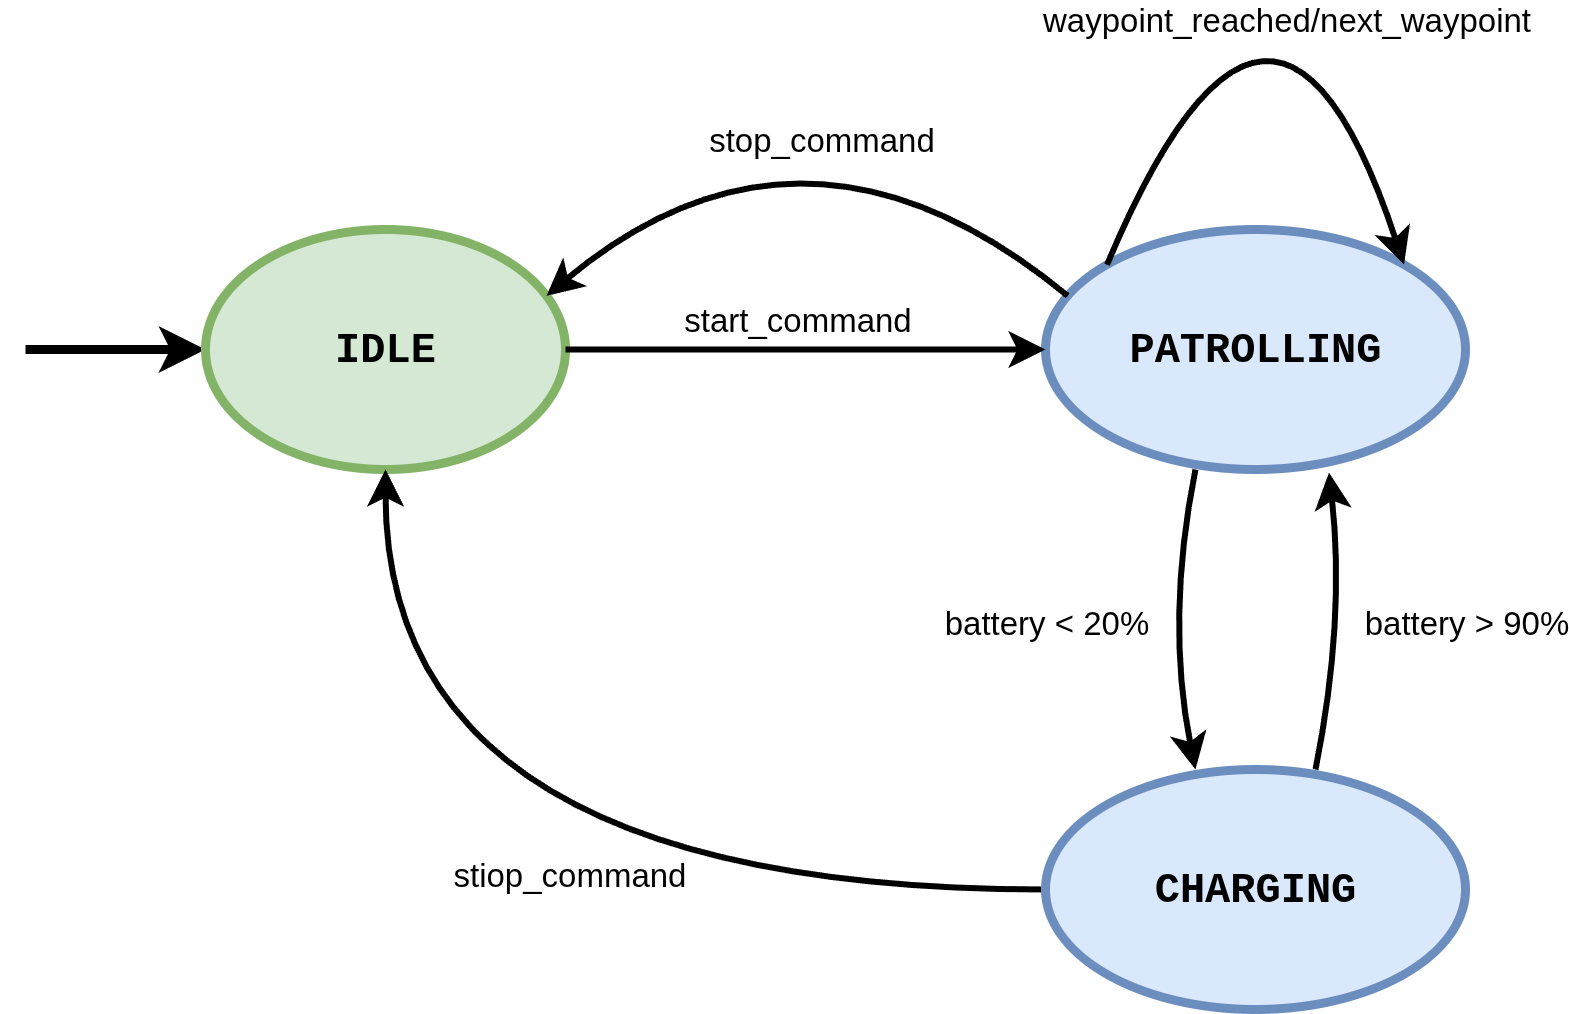
\includegraphics[width=0.97\linewidth,height=0.58\textheight,keepaspectratio]{images/tema_5/fsm_ejemplo_patrullaje.drawio.png}
  \end{column}
\end{columns}
\end{frame}

\begin{frame}{Elementos fundamentales de una FSM}
\small
\begin{itemize}
  \item \textbf{Estado:} modo de operación (ej. IDLE, SEARCHING, AVOIDING).
  \item \textbf{Transición:} cambio posible entre estados.
  \item \textbf{Evento:} disparador (mensaje, timeout, resultado de acción).
  \item \textbf{Guarda:} condición booleana para habilitar la transición.
  \item \textbf{Acción:} efecto asociado al estado o a la transición.
\end{itemize}
\vspace{1mm}
\small
Formalmente:
\[
\text{Transición} = \text{Evento} + [\text{Guarda}] / \text{Acción}
\]
\end{frame}

\begin{frame}{Anatomía de un estado en robótica}
\small
\begin{itemize}
  \item \textbf{on\_entry:} se ejecuta una vez al entrar (inicializa recursos).
  \item \textbf{on\_do:} se ejecuta cíclicamente (control y evaluación).
  \item \textbf{on\_exit:} se ejecuta al salir (parada segura y liberación).
  \item Este ciclo evita estados inconsistentes en actuadores y sensores.
\end{itemize}
\vspace{1mm}
\begin{center}
  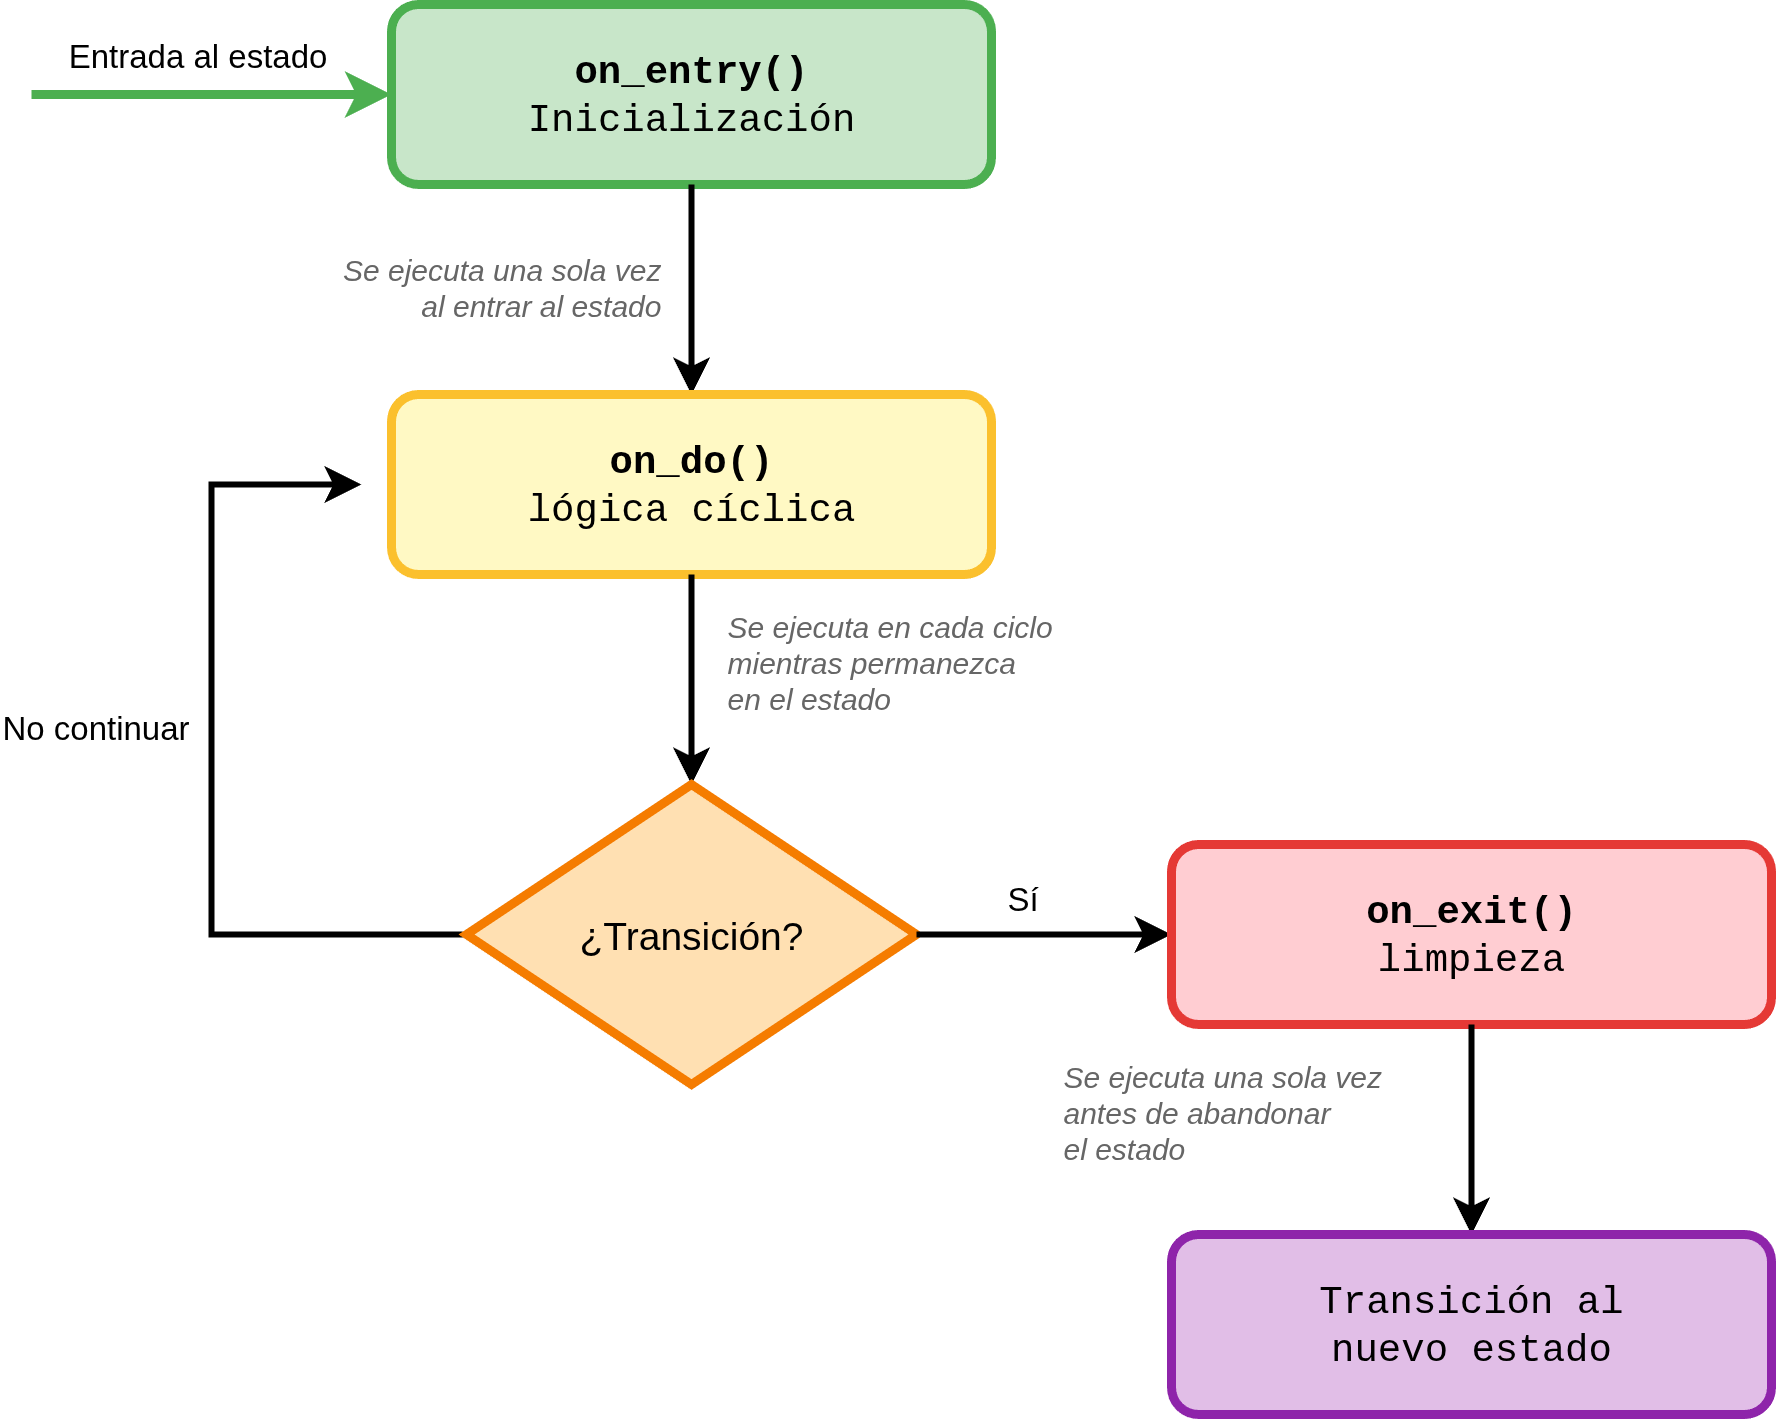
\includegraphics[width=0.78\linewidth,height=0.44\textheight,keepaspectratio]{images/tema_5/state_lifecycle.drawio.png}
\end{center}
\end{frame}

\begin{frame}{Moore vs Mealy}
\small
\begin{columns}[T,onlytextwidth]
  \begin{column}{0.50\textwidth}
    \textbf{Moore}
    \begin{itemize}
      \item La acción se ejecuta en el estado.
      \item Diseño más modular y legible.
      \item Normalmente añade 1 ciclo de latencia.
    \end{itemize}
  \end{column}
  \begin{column}{0.50\textwidth}
    \textbf{Mealy}
    \begin{itemize}
      \item La acción se ejecuta en la transición.
      \item Reacción más inmediata.
      \item Útil en eventos críticos (frenada, emergencia).
    \end{itemize}
  \end{column}
\end{columns}
\vspace{1mm}
\begin{center}
  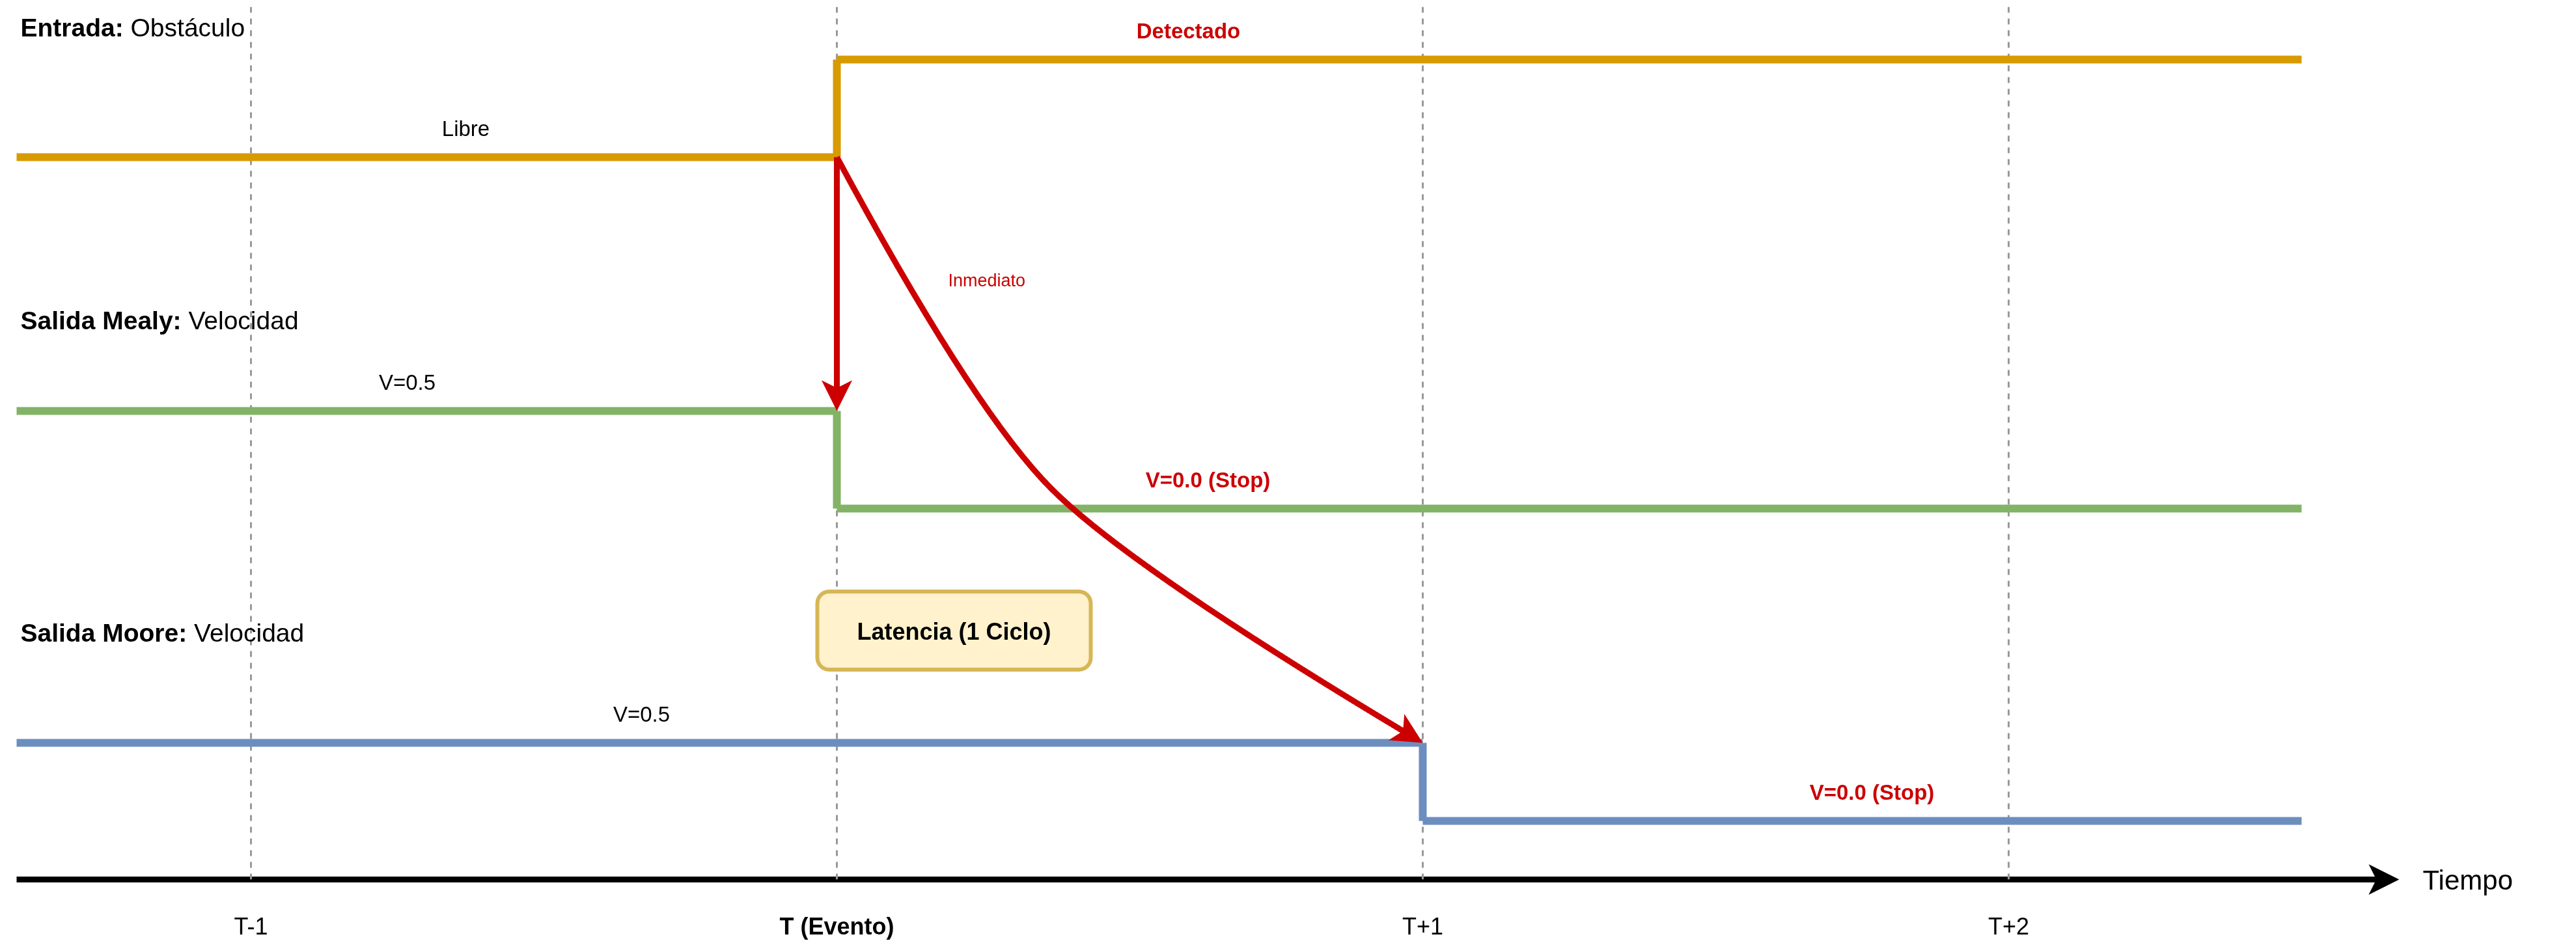
\includegraphics[width=0.95\linewidth,height=0.40\textheight,keepaspectratio]{images/tema_5/moore_vs_mealy.drawio.png}
\end{center}
\end{frame}

\begin{frame}{Concurrencia y explosión combinatoria}
\small
\begin{itemize}
  \item Una FSM clásica solo está en un estado cada instante.
  \item Si combinamos comportamientos independientes, el número de estados explota.
  \item Ejemplo: navegación (3) + batería (2) + luces (2):
  \[
    3 \times 2 \times 2 = 12
  \]
  \item Resultado: diagrama difícil de mantener y depurar.
\end{itemize}
\vspace{1mm}
\begin{center}
  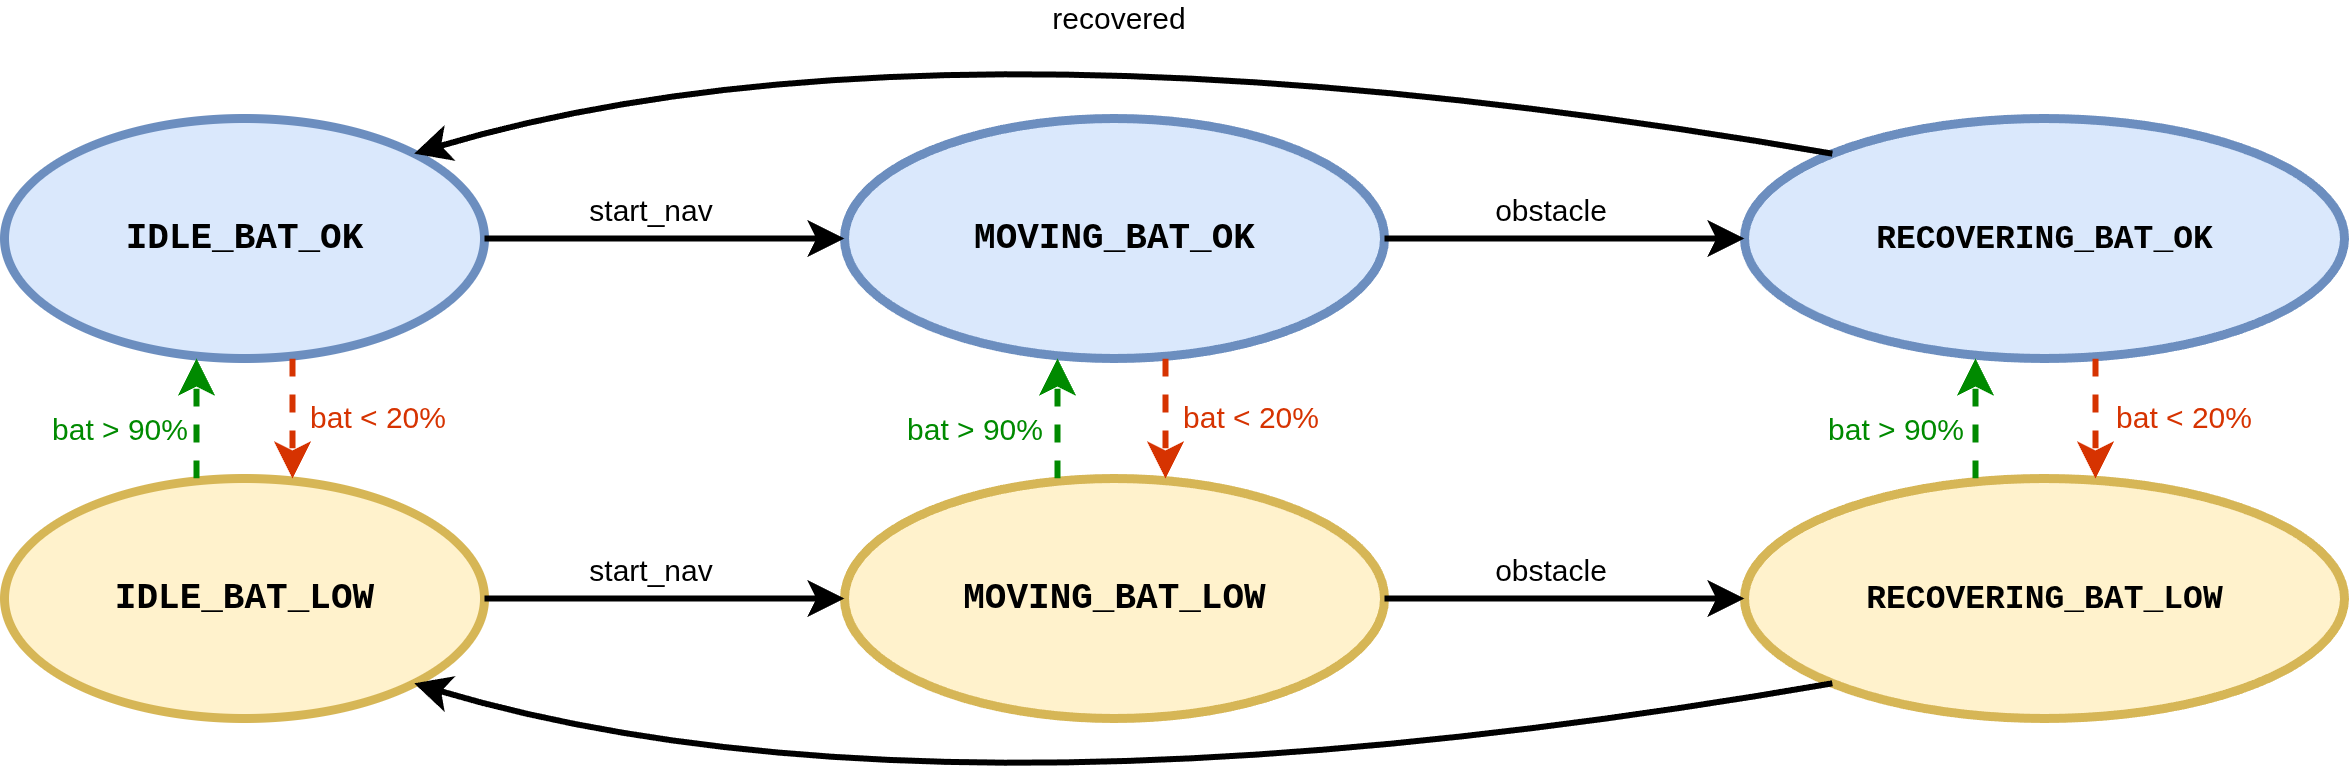
\includegraphics[width=0.95\linewidth,height=0.38\textheight,keepaspectratio]{images/tema_5/combinatorial_explosion.drawio.png}
\end{center}
\end{frame}

\begin{frame}{Statecharts: ortogonalidad y jerarquía}
\small
\begin{itemize}
  \item \textbf{Regiones ortogonales:} varias FSM pequeñas activas en paralelo conceptual.
  \item \textbf{Jerarquía:} un superestado puede contener subestados.
  \item Beneficios:
  \begin{itemize}
    \item menor complejidad,
    \item mejor modularidad,
    \item transiciones de emergencia factorizadas.
  \end{itemize}
\end{itemize}
\begin{columns}[T,onlytextwidth]
  \begin{column}{0.5\textwidth}
    \centering
    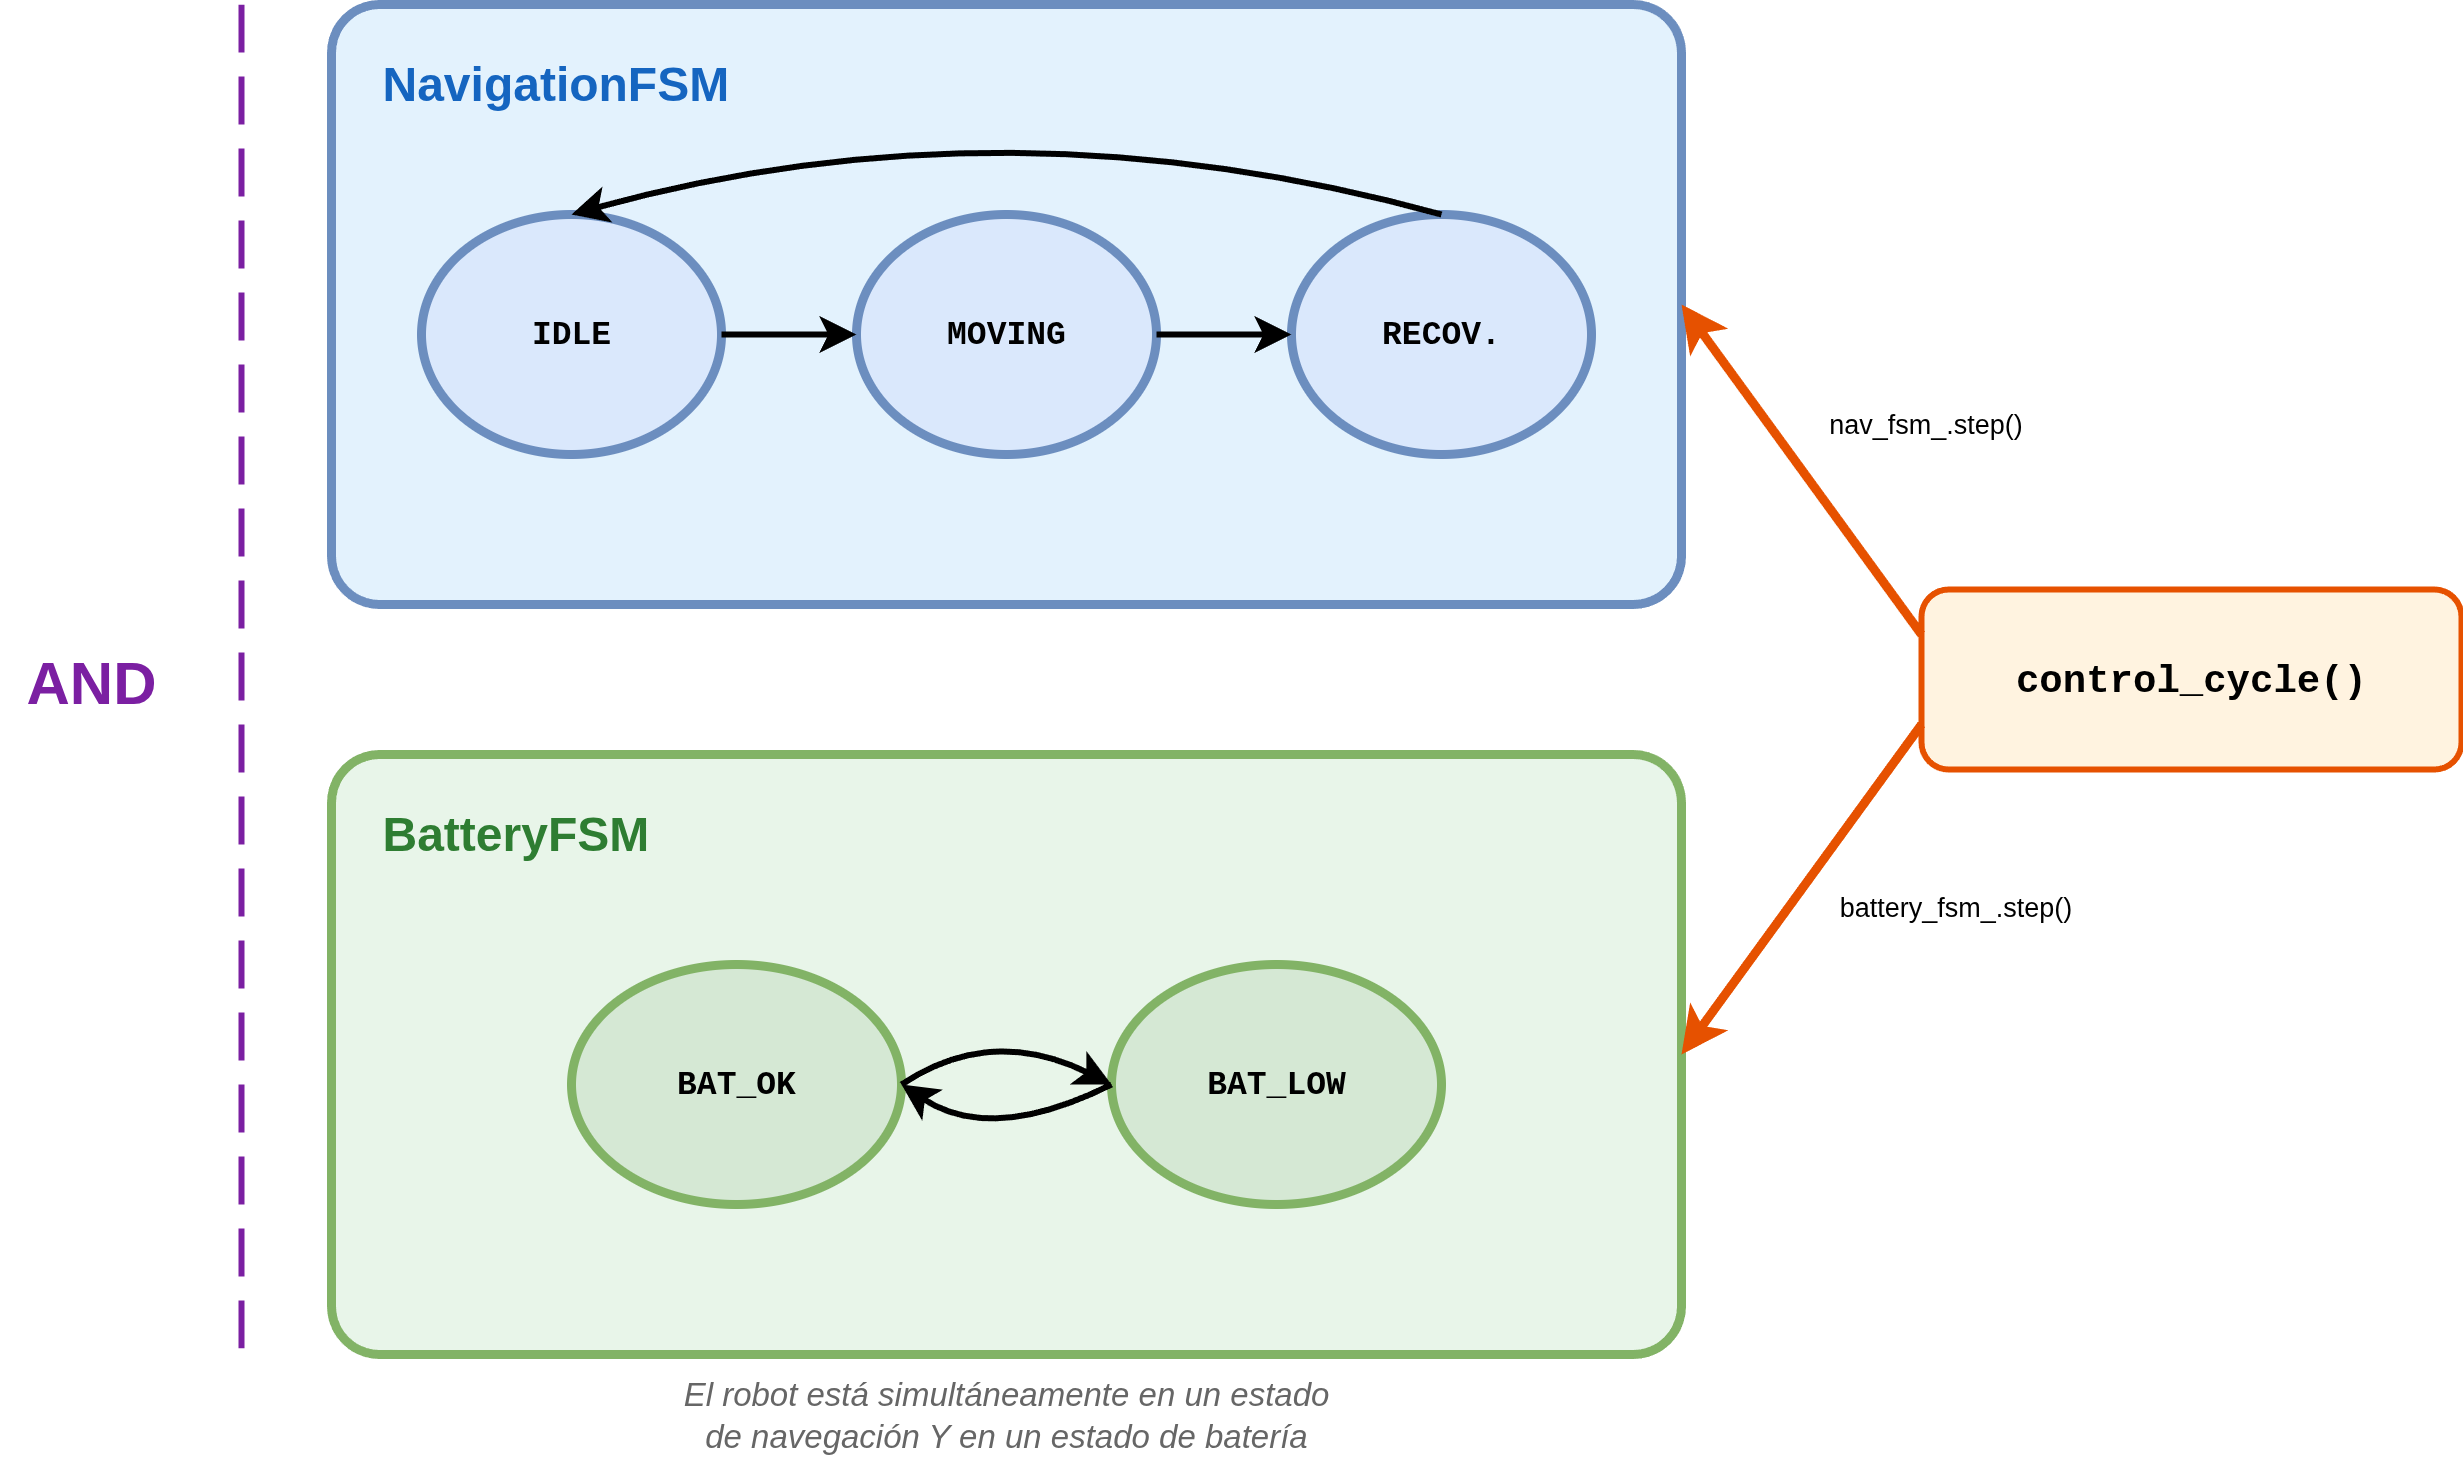
\includegraphics[width=0.98\linewidth,height=0.30\textheight,keepaspectratio]{images/tema_5/orthogonal_decomposition.drawio.png}
  \end{column}
  \begin{column}{0.5\textwidth}
    \centering
    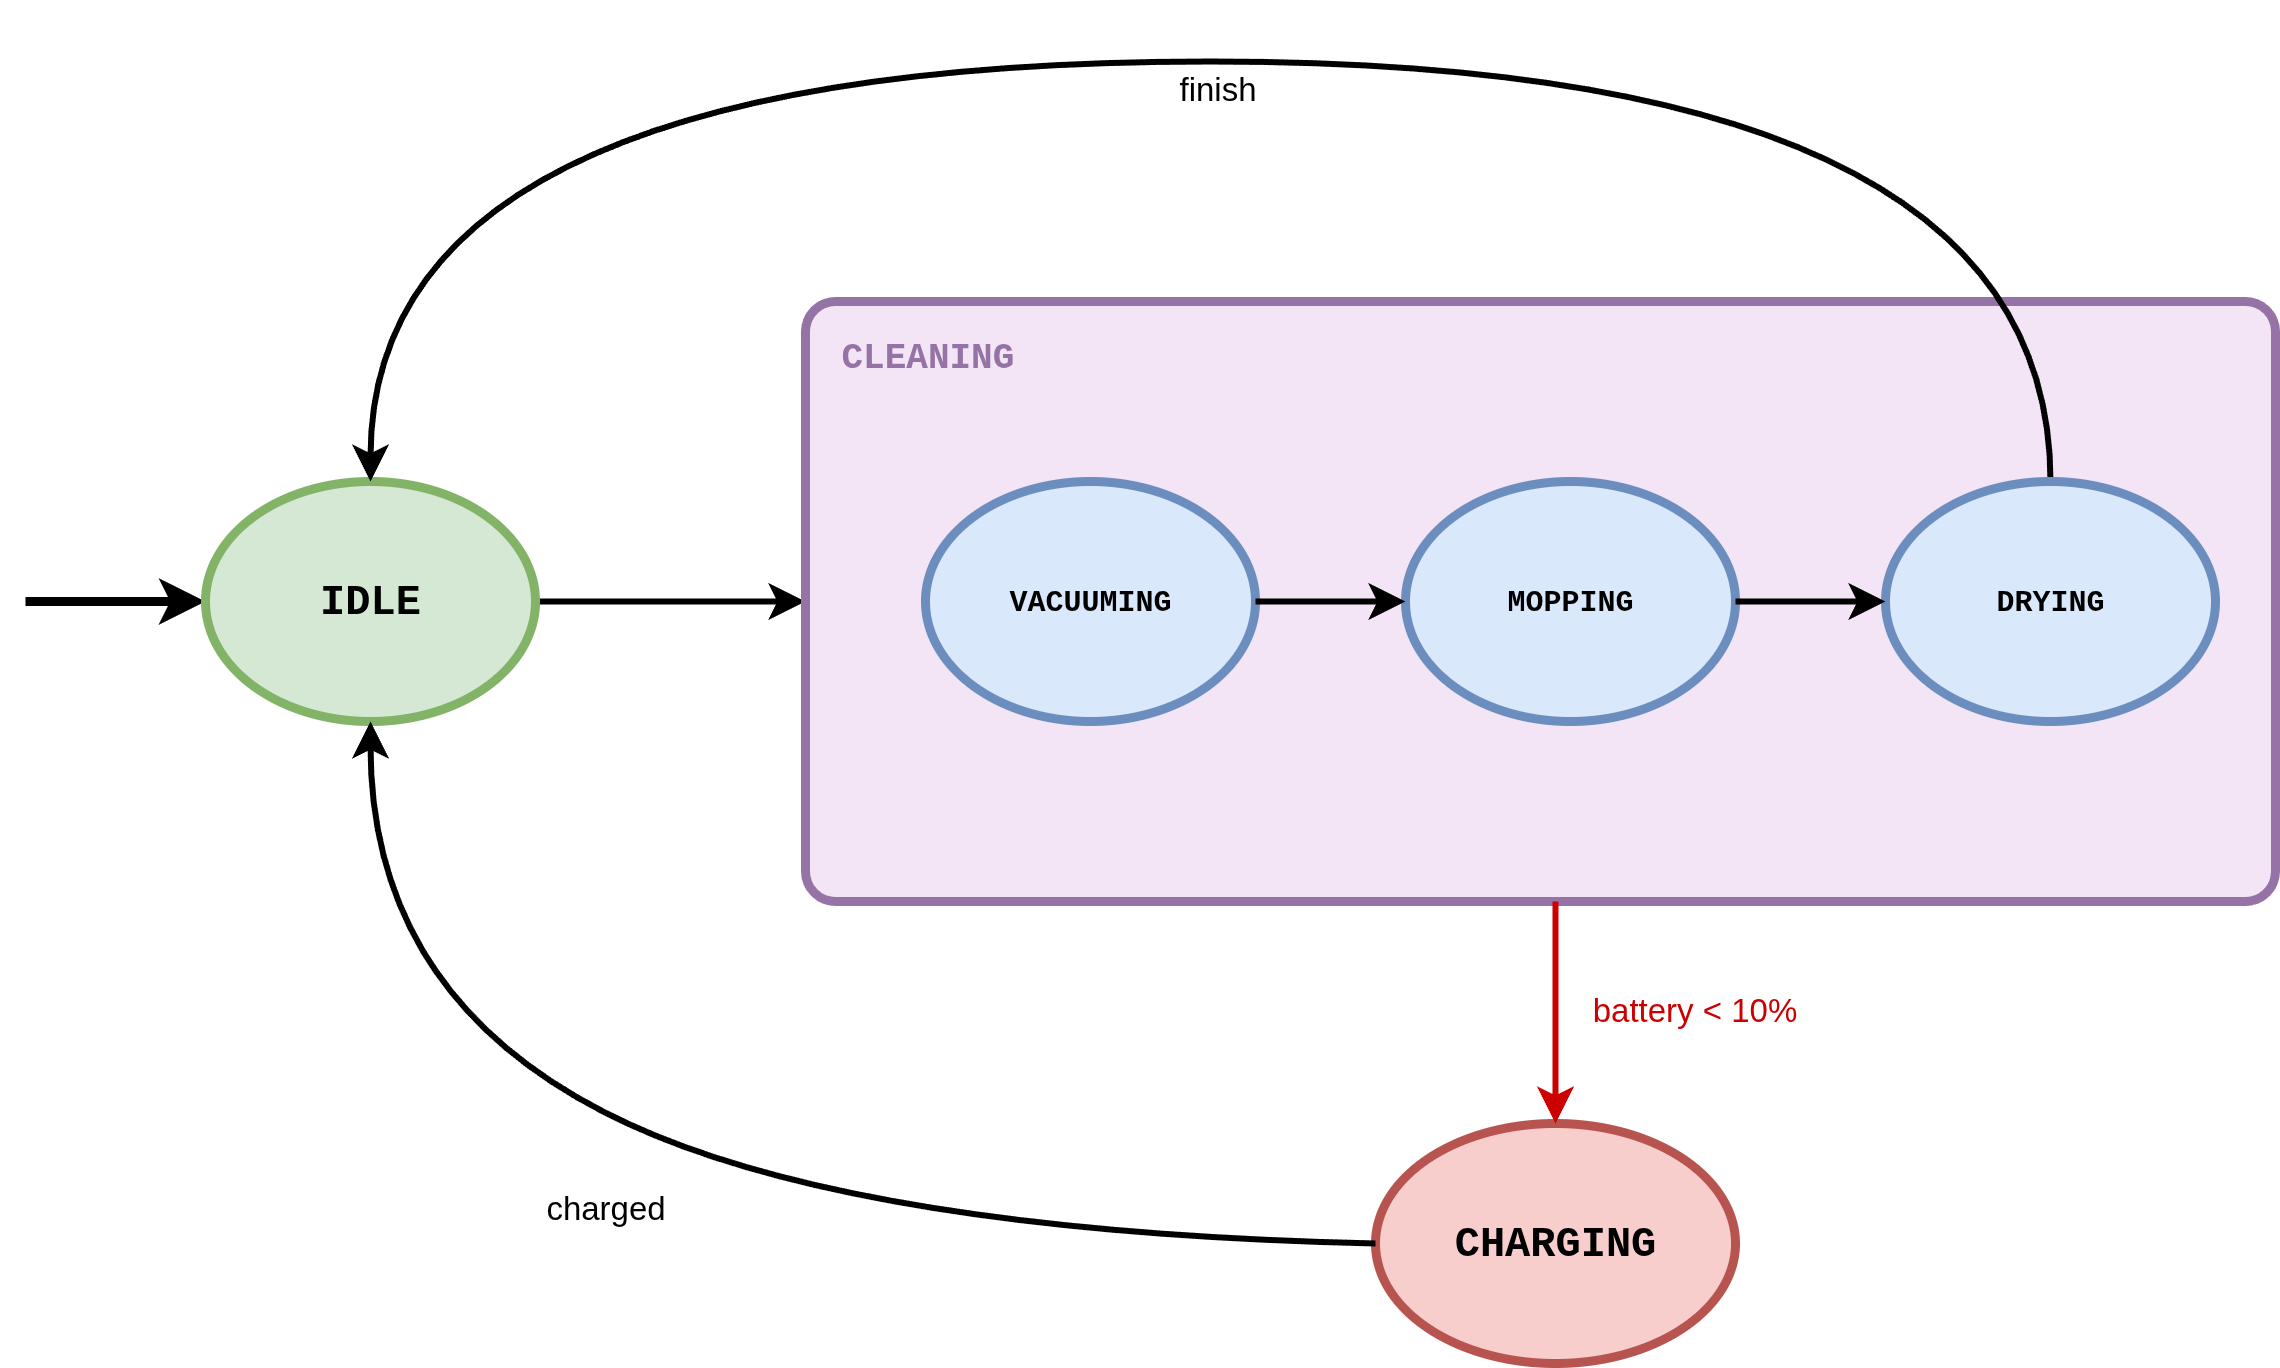
\includegraphics[width=0.98\linewidth,height=0.30\textheight,keepaspectratio]{images/tema_5/fsm_jerarquica_limpieza.drawio.png}
  \end{column}
\end{columns}
\end{frame}

%=================================================
\section{FSM en la arquitectura del curso}
%=================================================

\begin{frame}{FSM como alternativa en este curso}
\small
\begin{itemize}
  \item Propuesta didáctica: usar FSM para estructurar \textbf{misión} y flujo de decisión.
  \item Integración con arquitectura por capas:
  \begin{itemize}
    \item FSM de misión decide fase global,
    \item tareas coordinan ejecución,
    \item capacidades ejecutan acciones concretas.
  \end{itemize}
  \item Es compatible con otros enfoques:
  \begin{itemize}
    \item BT para tareas complejas,
    \item control clásico para bucles de bajo nivel.
  \end{itemize}
\end{itemize}
\end{frame}

\begin{frame}{Ejemplo de FSM de misión}
\small
\begin{itemize}
  \item Fases típicas: planificar, ejecutar, investigar anomalías y reportar.
  \item Las transiciones dependen de eventos del entorno y estado del sistema.
\end{itemize}
\vspace{1mm}
\begin{center}
  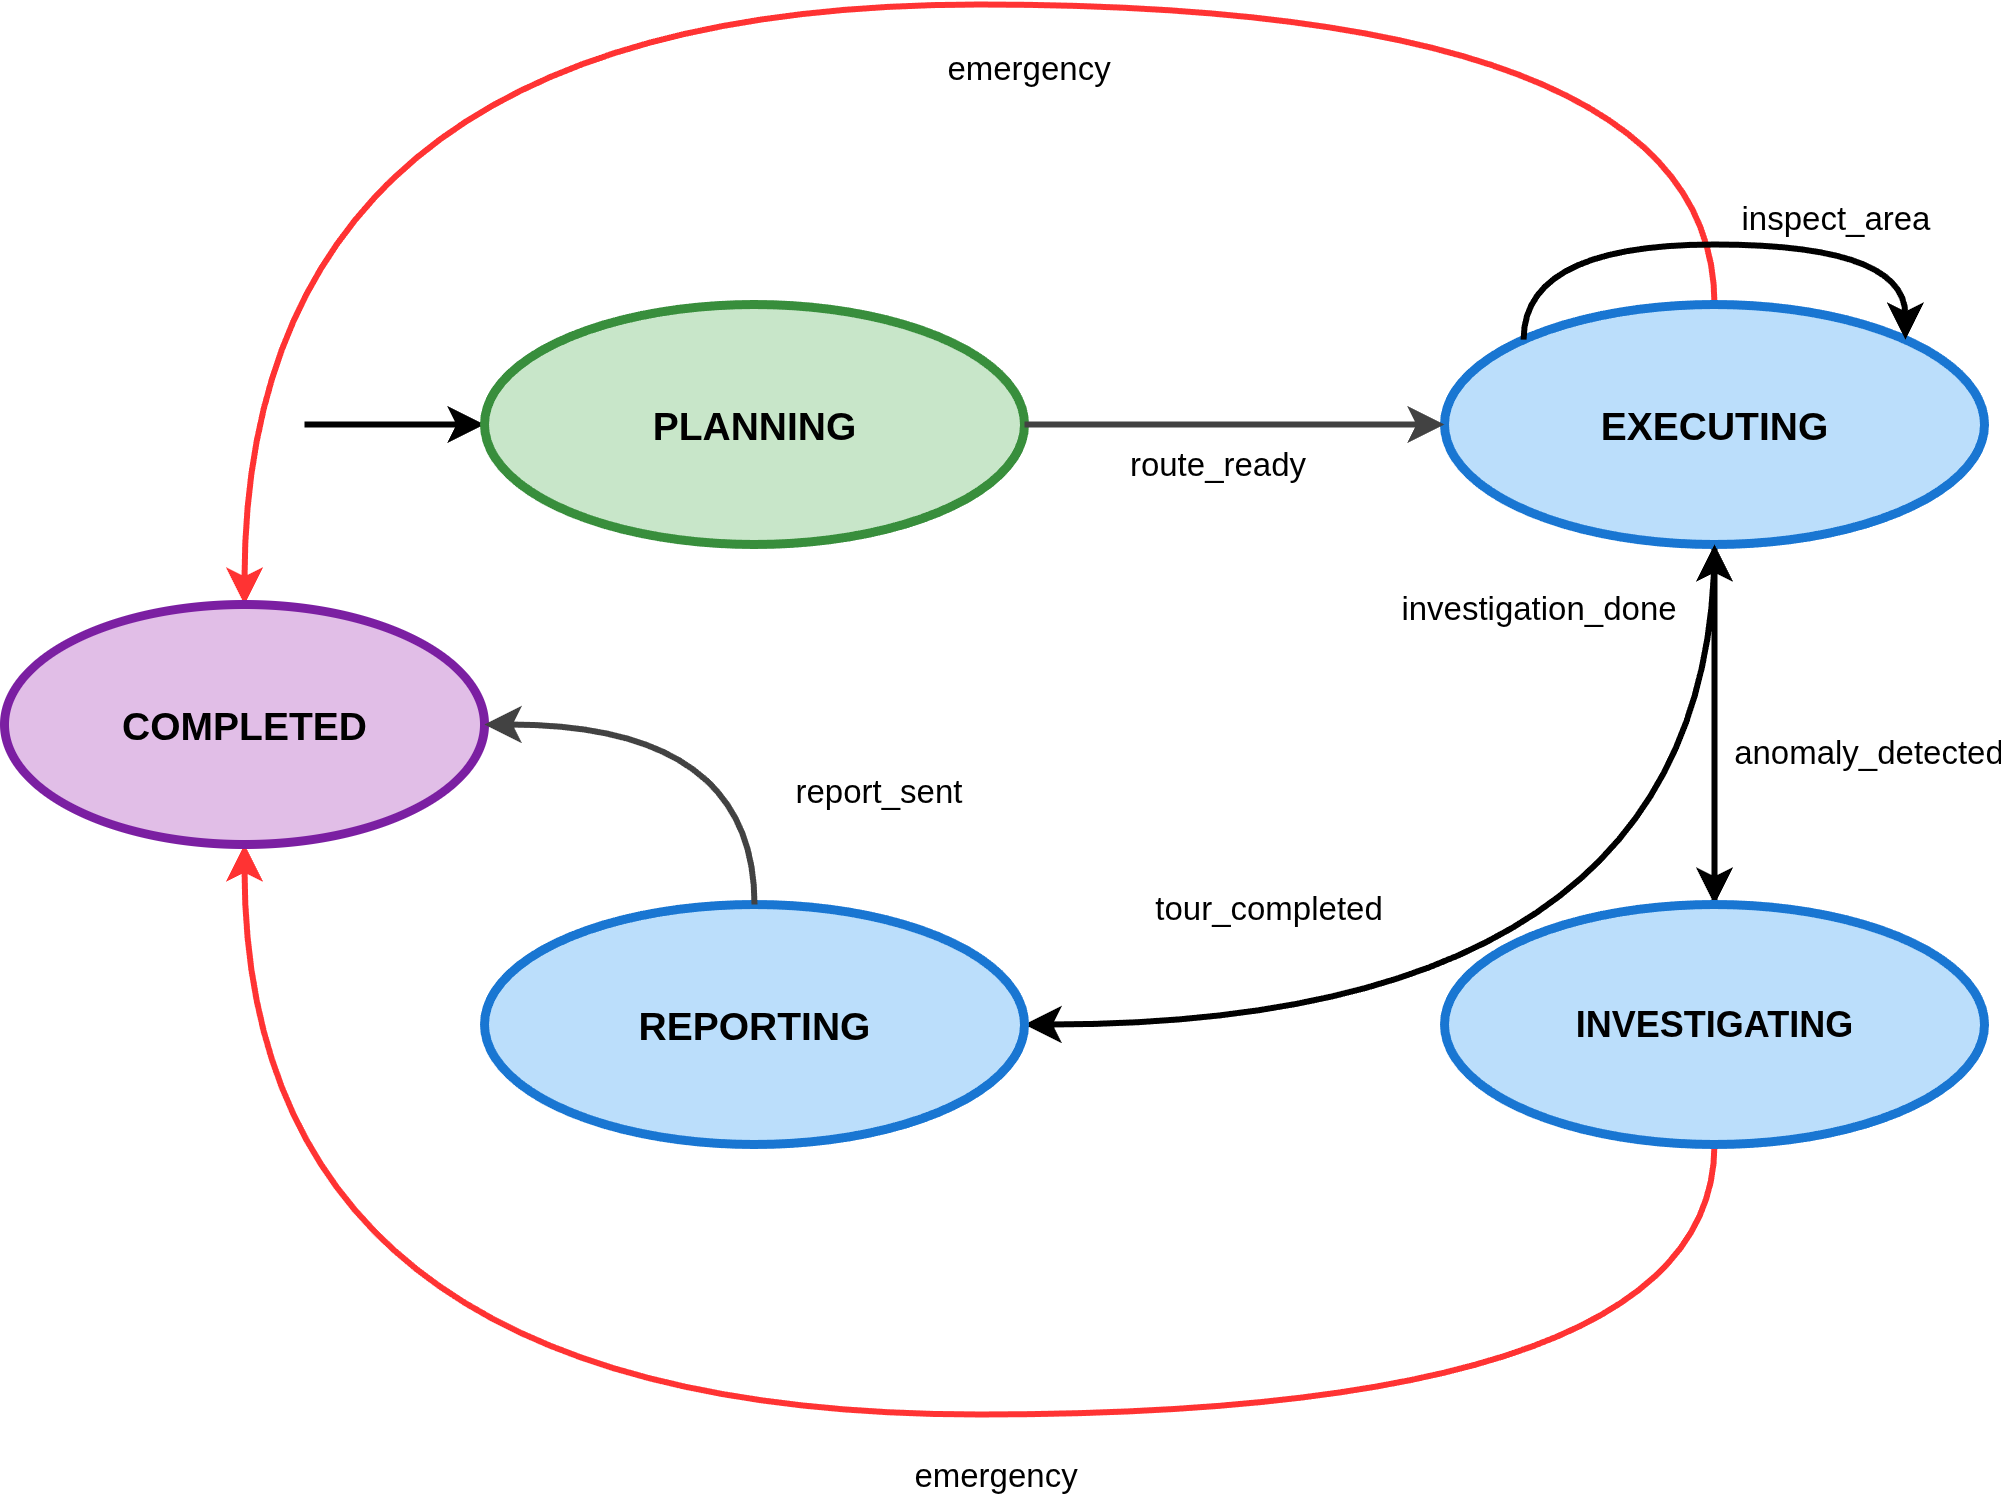
\includegraphics[width=0.82\linewidth,height=0.56\textheight,keepaspectratio]{images/tema_5/fsm_mision_inspeccion.drawio.png}
\end{center}
\end{frame}

\begin{frame}{Ejemplo de FSM de tarea}
\small
\begin{itemize}
  \item Tarea \texttt{TransportObject}: navegar, agarrar, transportar, soltar y recuperarse de fallos.
  \item La FSM decide secuencia y contingencias.
  \item Las capacidades ejecutan navegación y manipulación.
\end{itemize}
\vspace{1mm}
\begin{center}
  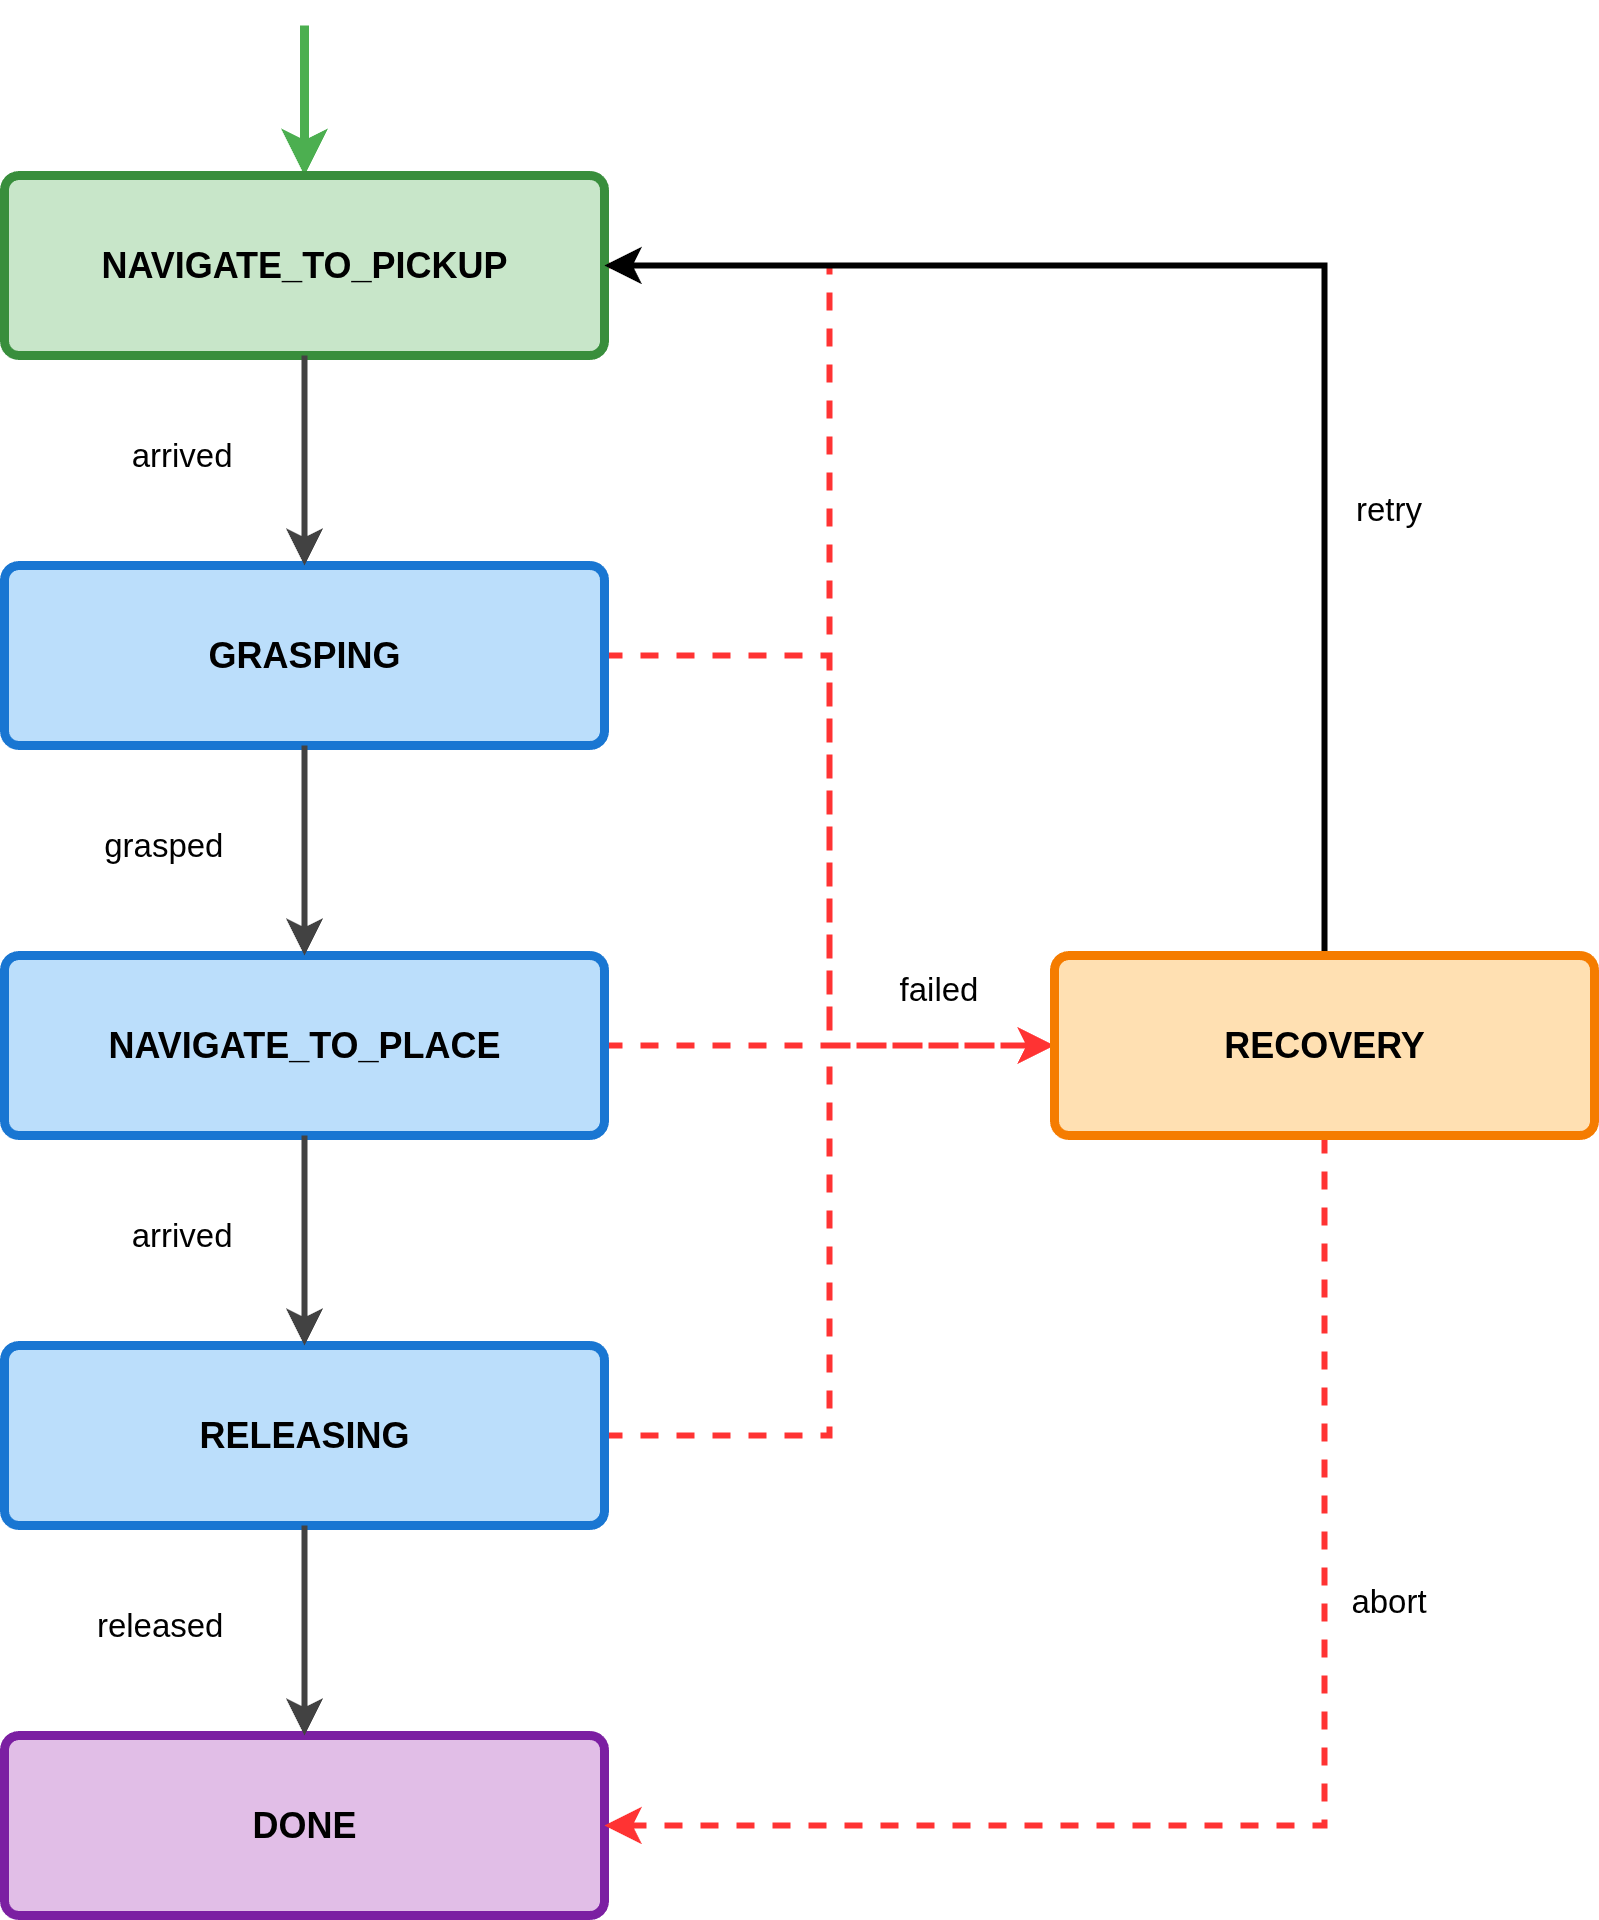
\includegraphics[width=0.72\linewidth,height=0.54\textheight,keepaspectratio]{images/tema_5/fsm_tarea_transporte.drawio.png}
\end{center}
\end{frame}

\begin{frame}{Composición misión--tarea--capacidad}
\small
\begin{itemize}
  \item La misión activa tareas.
  \item Cada tarea orquesta capacidades reutilizables.
  \item Se mejora trazabilidad, escalabilidad y mantenibilidad del comportamiento.
\end{itemize}
\vspace{1mm}
\begin{center}
  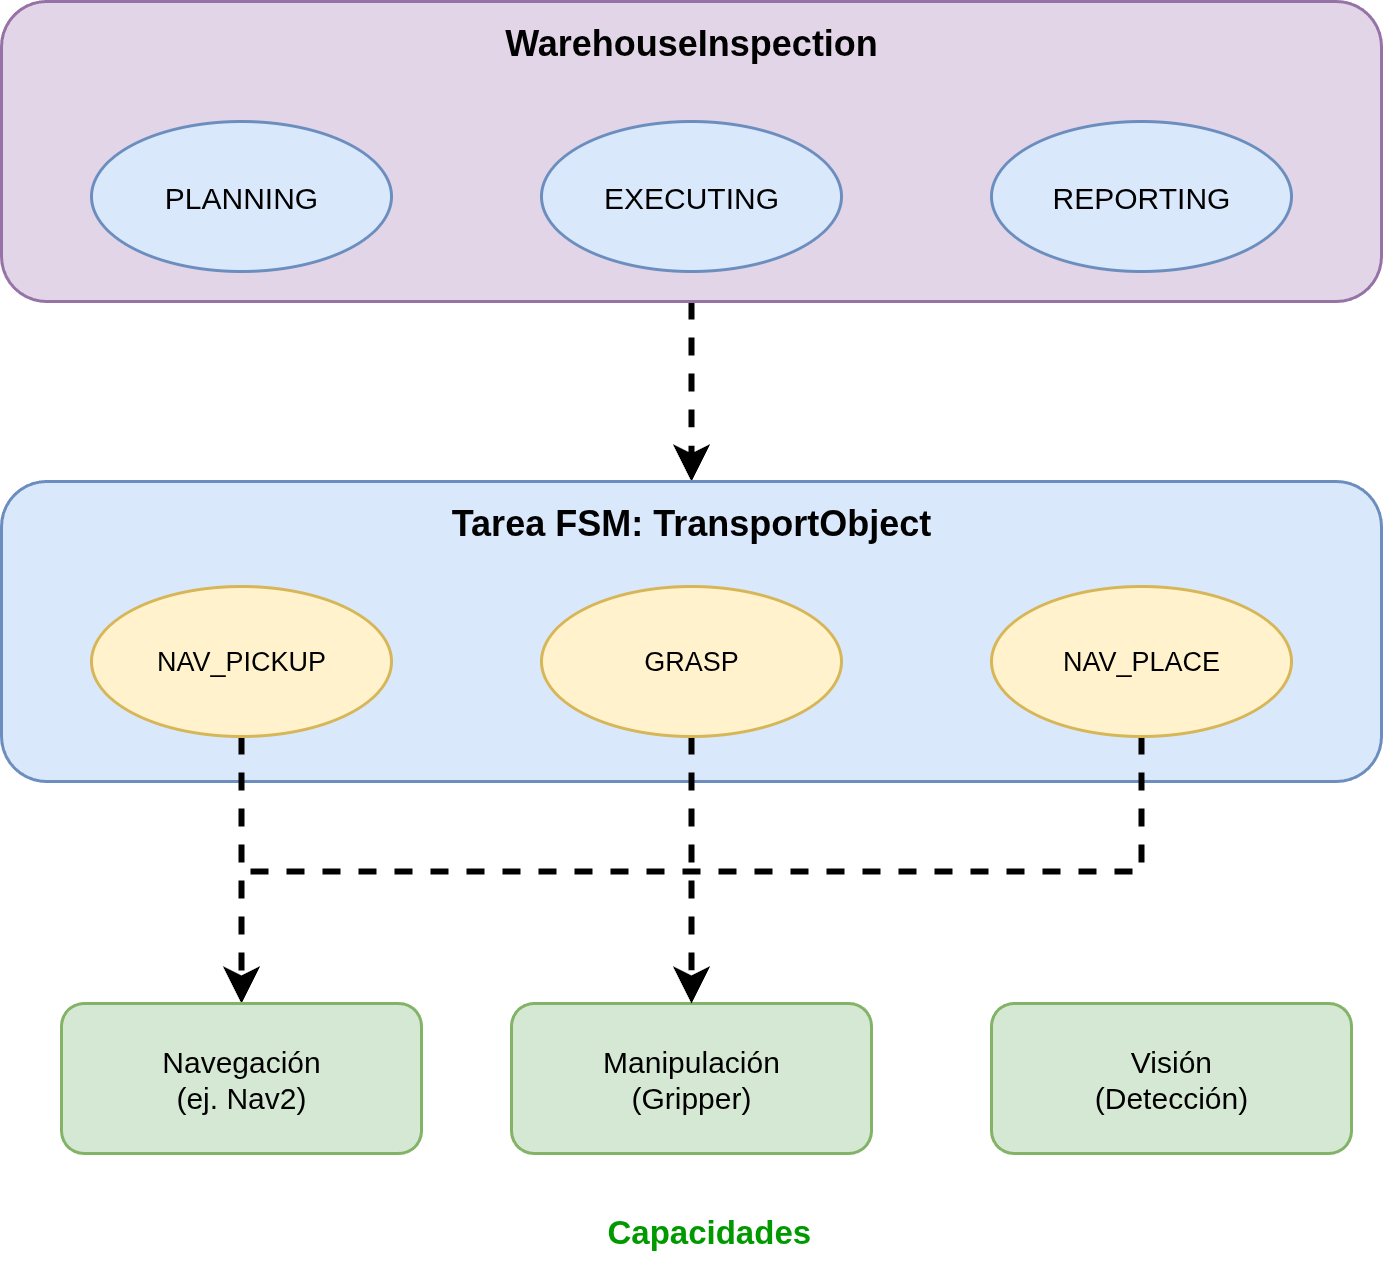
\includegraphics[width=0.82\linewidth,height=0.50\textheight,keepaspectratio]{images/tema_5/fsm_composicion.drawio.png}
\end{center}
\end{frame}

%=================================================
\section{Comparativa y cierre}
%=================================================

\begin{frame}{Control clásico vs FSM}
\small
\begin{columns}[T,onlytextwidth]
  \begin{column}{0.50\textwidth}
    \textbf{Control clásico}
    \begin{itemize}
      \item Excelente para seguimiento y regulación continua.
      \item Opera en bucles de bajo nivel (P, PI, PID).
      \item No modela bien fases discretas de comportamiento.
    \end{itemize}
  \end{column}
  \begin{column}{0.50\textwidth}
    \textbf{FSM}
    \begin{itemize}
      \item Excelente para modos y secuencias de decisión.
      \item Explicable y fácil de depurar a nivel lógico.
      \item Debe combinarse con control continuo en capacidades.
    \end{itemize}
  \end{column}
\end{columns}
\end{frame}

\begin{frame}{Conclusiones}
\small
\begin{itemize}
  \item Las FSM son una alternativa sólida para organizar el control de comportamientos.
  \item Hacen explícitas las decisiones del robot y su evolución temporal.
  \item Con ortogonalidad y jerarquía, escalan mejor que FSM planas.
  \item En este curso se usan como puente entre sistemas reactivos y arquitecturas deliberativas.
  \item La práctica recomendada: FSM para decisión + capacidades con control continuo.
\end{itemize}
\end{frame}

\begin{frame}
  \centering
  \Large Preguntas
\end{frame}

\end{document}
